%%%%%%%%%%%%%%%%%%%%%%%%%%%%%%%%%%%%%%%%%%%%%%%%%%%%%%%%%%%%%%
% Titel
%	Autor: Lukas Baronyai
%%%%%%%%%%%%%%%%%%%%%%%%%%%%%%%%%%%%%%%%%%%%%%%%%%%%%%%%%%%%%%
\documentclass[pdftex,a4paper,10pt]{article}
%%%%%%%%%%%%%%%%%%%%%%%%%%%%%%%%%%%%%%%%%%%%%%%%%%%%%%%%%%%%%%
%Standardformatierung
\usepackage[left=3cm,right=3cm,top=2cm,bottom=1.5cm,includefoot]{geometry}
\usepackage[USenglish]{babel} 
\usepackage[ansinew]{inputenc}
%für Silbentrennung und Schriftstil
\usepackage[T1]{fontenc}
\usepackage{lmodern}
%für diverse Figuren
\usepackage{graphicx}	%für Bilder/Grafiken einbinden
\usepackage{booktabs} %schönere Tabellen
\usepackage{wrapfig}  %mit oder von Schrift umflossen Bilder
%für Mathe
\usepackage{amssymb}
\usepackage{amsmath}
\usepackage{amsthm}
\usepackage{amsbsy}
\usepackage{amsfonts}
\usepackage{amstext} %\text für Math-Umgebung
%Referenzen
\usepackage{prettyref} %eigene Ref mit \newrefformat
\usepackage{hyperref} %klickbare Verweise
\usepackage{url}	%URL-Links
%Algorithmen
\usepackage[]{algorithm2e}
\usepackage{algpseudocode}
%anderes Zeug
\usepackage{grffile} %pdf-Files mit Leerzeichen einbinden
\usepackage{microtype}	%schönere pdfs
\usepackage[multiple]{footmisc}  %für Fußnoten
\usepackage{csquotes}
\usepackage[final]{pdfpages}
\usepackage[numbers]{natbib}
\usepackage{pgfplots}
\usepackage{subfigure}
\usepackage[titletoc,toc,title]{appendix}
\usepackage{array,booktabs}% http://ctan.org/pkg/{array,booktabs}
\renewcommand{\arraystretch}{1.5}% Spread rows out...
%%%%%%%%%%%%%%%%%%%%%%%%%%%%%%%%%%%%%%%%%%%%%%%%%%%%%%%%%%%%%%
\setcounter{page}{1}			%setzt erste Seitennummer auf 1(falls Titelblatt nicht gezählt werden soll)
\setcounter{secnumdepth}{3}	%setzt Kapitelnummerierungstiefe auf 6
\setcounter{tocdepth}{3}			%Kapitelnummerierungstiefe für Inhaltsverzeichnis
\makeindex
%%%%%%%%%%%%%%%%%%%%%%%%%%%%%%%%%%%%%%%%%%%%%%%%%%%%%%%%%%%%%%
\begin{document}
\pagestyle{plain}
\setlength{\tabcolsep}{10pt}
\pagenumbering{gobble}
%%%%%%%%%%%%%%%%%%%%%%%%%%%%%%%%%%%%%%%%%%%%%%%%%%%%%%%%%%%%%%
\title{Linked~Open~Data\\
	   at the\\
	   Vienna~University~of~Technology\\
	   \large A case study about research data}
\author{Lukas Baronyai$^a$, \textit{Author}\\
		Kevin Haller$^b$, \textit{Co-Author}\\
		Stefan Gamerith$^c$, \textit{Co-Author}\\
	\texttt{\{e1326526$^a$,kevin.haller$^b$,e0925081$^c$\}@student.tuwien.ac.at}}
\date{\today}

\maketitle

\begin{abstract}
The abstract goes here.
\end{abstract}

\vfill
\begin{center}
\textbf{Keywords.} Linked Open Data, University, Case Study
\end{center}

%%%%%%%%%%%%%%%%%%%%%%%%%%%%%%%%%%%%%%%%%%%%%%%%%%%%%%%%%%%%%%
\newpage
\tableofcontents
%\newpage
\cleardoublepage
\listoffigures
\pagenumbering{arabic}
%%%%%%%%%%%%%%%%%%%%%%%%%%%%%%%%%%%%%%%%%%%%%%%%%%%%%%%%%%%%%%

\section{Introduction}
While the pressure on governments and public organizations to release \textit{Open Data~(OD)} has significantly grown with the spread of information systems there has been also a need for \textit{linking} these data from various sources to understand the information in a contextual sense.

As OD includes non-confidential data any restrictions in distribution are prohibited and information is funded only by public money~\cite{article:janssen2012benefits}. The application domain for OD providers is not restricted by its nature in any way including from traffic, weather and public transport to name a few. However, exclusively exposing public assets is not enough, in addition establishing a feedback loop facilitates an ongoing adaption to the stakeholders concerns. 

The World Wide Web has proven great success in spreading knowledge of various data sources all over the world. The building blocks of the Web are documents and links building a shared, global and connected information source. This can be seen as the key success factor in its nearly unconstrained growth~\cite{report:jacobs-i-2004--a}. 
\textit{Linked~Data~(LD)} has adopted these principles of publishing and connecting data realized as machine-readable, structured data connected to various data sets which in turn are linked to different data sets. 

\citet{article:bernerslee_2006} developed a five star deployment scheme classifying OD. The scheme ranges from a one star rating covering proprietary data formats~(e.g. Portable Document Format~(PDF)) to a five rating including machine-readable formats using open standards with links to other data sets.

Although LOD offers universities new opportunities for providing unprecedented insight into its core activities and ease application development, a major \textbf{problem} is that \textbf{LOD has not been widely adopted by universities yet}. Even though there are a few examples~\cite{url:linked-universities-members} of publishing university related data sets as LOD there has been little knowledge of its usage for publishing university related information. 

To answer the research questions stated in the next sub-section we conducted interviews at the Vienna University of Technology. In particular \textbf{the context of this work are research data}, though there exist papers investigating similar research questions but with different context:~\citet{article:gamerith_publishing_2016} (administration data) and ~\citet{article:haller_publishing_2016}(data concerning students). 

The remainder of this section states the addressed research questions, describes the contributions of this work and gives an overview of the structure of this paper.

\subsection{Research Questions}
The fundamental research question we investigate is:
\begin{displayquote}
\textit{How can Linked~Open~Data help to improve processes in a university context and how can it be successfully applied?}
\end{displayquote}
More concrete, this paper concentrates on the following four research questions:
\paragraph{RQ1: What are best practices regarding the applicability of Linked Open Data in university settings?}
At the time of writing this paper there are no established best practices for the use of LOD due to its little adoption in university settings. For this very reason it is crucial to identify strengths and limitations from previous experiences of using LOD as the foundation of information systems~\cite{url:linked-universities-members}. 
\paragraph{RQ2: What are major benefits and barriers for each stakeholder and what are useful use cases?}
We identified three different stakeholders \textit{Students}, \textit{Researchers} and \textit{Administration staff}.
However, focus of this work are researchers.
Since the success of any new technology highly depends on their acceptance concerns of each target group needs examination. Furthermore, use cases are important to showcase profits and shortcomings. 
\paragraph{RQ3: What are major challenges for the implementation of a Linked Open Data solution?}
As the implementation of a LOD solution is a time consuming task the knowledge of probable challenges from a technical perspective as well as from a management perspective is key to a successful adoption. 
\paragraph{RQ4: How would a prototypical implementation of a publication framework based on Linked~Open~Data look like?}
Among the definition of building blocks for a publication framework of university related assets a high level picture of the overall architecture needs to be drawn to give implementers and LOD experts a common understanding of the system. Next, defining sample ontologies representing selected assets of the university domain draws concrete examples of how LOD data might look like. 

\subsection{Methodology}
Finding an answer for the research questions above has led to the following three methodologies:
\paragraph{A coordinated set of semi-structured interviews}
To answer research questions RQ2-RQ4, we interviewed a selected set of \textit{researcher}. Semi-structured interviews were selected as the means for data collection because they are well suited for exploring the impressions and interests of the interviewees like in a discussion while still following a defined structure. 
\paragraph{Literature Review}
Undertaking a literature review to justify scientific contributions and making sound conclusions is an established practice in any scientific community. Since our scientific work targets to the Semantic Web community we made some pre-assumptions about a basic understanding of the technologies and concepts used in that respective area. More specifically, we assume a basic understanding of the concept of an ontology and some pre-knowledge about ontology description languages. 
\paragraph{Conceptual System Design}
The development of applications based on LOD requires a methodology facilitating a common understanding of the overall system infrastructure. Therefore we designed a conceptual model of a prototypical implementation of a publication framework based on LOD. 

\subsection{Contributions}
The work in this paper mainly contributes to different aspects which need to be considered when designing and implementing an application driven by LOD.
More precisely, our contributions can be categorized into the following four areas:
\paragraph{1. Identifying best practices for Linked Open Data in university settings.}
Information systems needs to cope with vast amount of data nowadays growing the need to efficiently handle Linked Data as well. We gave a brief overview of existing research work in that area, in particular, we compared the benefits and shortcomings in existing LOD solutions. 
\paragraph{2. Finding benefits/barriers including additional use cases for stakeholders.}
As with every software project the very first phase of the Software Development Lifecycle~(SDLC) is \textit{evaluating of requirements}. As LOD driven software has additional requirements to the accessibility of data and their organization we investigated if the overhead compared to an established technology~(e.g. a database based solution) is feasible. A set of selected \textit{researcher} are interviewed at the Vienna University of Technology. Additionally we proposed several use cases emphasizing their point of view. 
\paragraph{3. Discovering possible obstacles for implementers of a Linked Open Data solution.}
As the application domain for a Linked Data is limited to the university context our work includes LOD driven applications resulting from our conducted interviews.
\paragraph{4. Sketching a prototypical implementation of a publication framework driven by Linked Open Data.}
The proposed publication framework covers the whole process of data provision, requirement analysis and application development designed for but not limited to university related assets.  
\subsection{Structure of this Paper}
\%\%\%\%tbd\%\%\%\%
\section{Related work}
\subsection{Linked Universities}\label{linkeduniversities}
One of the most important university projects in the world of LD are the LinkedUniversities. They are "`\textit{an alliance of european universities engaged into exposing their public data as linked data}"'\citet{url:linkeduniversities}, providing help and knowledge for other universities who wants to implement LD-Systems in their infrastructure. Addressing the problem of connecting data and developing new sites by inexperienced universities, the alliance provide information so they don't have to be re-learned. For this purpose the LinkedUniversities offering a portal as collaborative space with common vocabularies and practices for reusing, describing and sharing.

Their goals are:~\footnote{\citet{url:linkeduniversities}}

\begin{itemize}
\item "`Identify, support and develop common linked data vocabularies, usable accross universities for common concepts such as courses, qualifications, educational material, etc."'
\item "`Describe reusable recipes, and share reusable tools, for exposing linked data in universities"'
\item "`Support, through experience sharing and reuse, initiatives towards exposing university data as linked data"'
\end{itemize}


The members of this alliance are:(~\footnote{\citet{url:linked-universities-members}})
\begin{itemize}
	\item The Open University, UK
	\item University of M\"unster, Germany
	\item Aalto University, Finland
	\item University of Southampton
	\item Royal Institute of Technology (KTH) / MetaSolutions AB
	\item Aristotle University of Thessaloniki, Greece
	\item Ege University, Turkey
	\item Charles University in Prague
	\item Universitat Pompeu Fabra
\end{itemize}

\subsubsection{Example: The Open University and the LUCERO Project}
LUCERO (Linking University Content for Education and Research Online) was a project from the Open University, funded for 1 year by the JISC Information Environment 2011 Programme under the call Deposit of research outputs and Exposing digital content for education and research. Aim of the project was to "` \textit{ scope, prototype, pilot and evaluate reusable, cost-effective solutions relying on linked data for exposing and connecting educational and research content}"'~\footnote{\citet{url:lucero}}. The projects connected with other organizations through LinkedUniversities.org to gather common issues and practices. They outcome was the first university linked data platform, \url{http://data.open.ac.uk/}, with much impact on The Open University and the education community.

\%\%\%\%TODO: section about Open Research Online\%\%\%\%

\subsection{Austrian Open Data}
\subsection{Linked Data for Libraries (LD4L)\label{ld-libraries}}

\%\%\%\%tbd\%\%\%\%

\subsection{Earlier studies}
\begin{itemize}
	\item Interlinking educational Resources and the Web of Data - a Survey of Challenges and Approaches (http://linkeduniversities.org/)
	\item a few more at http://linkeduniversities.org/lu/index.php/publications/index.html
	
	
\end{itemize}
\section{Benefits and Challenges using LOD (RQ2 \& RQ3)}~\label{section:benefits}
As mentioned in the introduction, we identified \textit{students}, \textit{researchers} and \textit{administration employees} as import stakeholders at a university. This chapter describes the methodology and results of the conducted case study involing researcher. The essential question of the case study was RQ2 (``\textit{What are major benefits and barriers for each stakeholder and what are useful use cases?}'') and RQ3 (``\textit{What are major challenges for the implementation of a Linked Open Data solution?}'') 
A case study concerning students was conducted by Kevin Haller~\cite{article:haller_publishing_2016} and another one concerning administration employees by Stefan Gamerith~\cite{article:gamerith_publishing_2016}.

The first section of this chapter describes the applied methodology (see section~\ref{subsection:methodology}). The second section evaluates and analyzes the results of the case study, investigating the possible benefits, barriers and challenges of some use cases and a general view at the interviewees (see section~\ref{subsection:results}).

\subsection{Methodology}
In this study the data were acquired by a coordinated set of semi-structured interviews. As mentioned the stakeholders were classified into three groups (\textit{administrative staff}, \textit{students} and \textit{researchers}) and therefore three different versions of the questionnaire but with joint parts for statistically evaluation were worked out. For each version exists an according paper, in this work only the category "`researcher"' will be described.

\subsubsection{Design of questionnaire}
The main purpose of the interviews were the collecting of the stakeholders thoughts, needs and knowledge, so the method of of a semi-structured interview was chosen. A \textit{fully structured interview} would not be adequate because of it's strict character allowing only predefined answers and a \textit{unstructured interview} would be to difficult to analyze.

After choosing the method, the questionnaire was defined. To allow a general, generic shared analyze of the interviewees the team decided to mix open questions from the semi-structured model with closed questions with fixed, predefined questions. The result had four parts:

\begin{enumerate}
	\item General question about the interviewee for classification, about his/her work
	\item General question about the interviewee's knowledge in general technical and LOD context. This part is the part for statistical evaluation.
	\item Explanation of LD, followed by a specific set of questions targeting the thoughts and opinions of the interviewee about presented use cases and example application. Motivation of this part is to introduce the interviewee to LOD if it is an unknown topic and let him/her start to think about LOD to prepare the next part
	\item Wide open Questions to explore and find use cases and existing data sources for LOD application at the university.
\end{enumerate}

The examples from part 3 were LD in libraries (see~\ref{ld-libraries}) and an obvious source of research related data: the publication database.

\subsubsection{Description of interviewed people}
As mentioned the interviewees of this study were chosen according to the category "`\textit{Research}"', so the interview partner were active researcher in various fields. Altogether four interviews were done. Because of the technical character of LOD the chosen people are all technically experienced so they are able to imagine use cases at the university. In future work there is a need of more less experienced researchers to understand their thoughts.

\subsubsection{Data Validity and Quality}
To ensure both a continuous conversation flow and a high quality recording of the spoken words, the interviews were held in teams, one speaker and one writer making notes. Additional all interviews were audio recorded.
As result the data are available as interview notes and audio records.
\newpage
\subsection{Results}\label{results}
After giving a detailed description of the used methodology in the previous subsection this subsection contains the interviews outcome. First the general questions about the interviewees background are evaluated and interpreted. Because this part was included in all three questionnaires, this part also includes data from the other reports for comparing the data, but only the data from the researcher interviews are interpreted. In the next parts, the use case of the library data and publication data are evaluated and their potential benefits, barriers and disadvantages analyzed. In the last part, the ideas and mentions from the open questions are evaluated.

\subsubsection{General statistically evaluation of the interviewees background}\label{stat_general}

\begin{figure}[htbp]
\centering
\label{Fi:lod-exp}
	\begin{tikzpicture}
		\begin{axis}
			[title=Level of ICT-Expertise,
			ybar,% Balken
			% urspr�ngliche y-Werte unterhalb der Balken:
			nodes near coords,nodes near coords align=above,point meta=rawy,
			axis x line=bottom, axis y line=left,% Achsen nur unten und links,
			%xlabel=blub,ylabel=bla, % Beschriftung der Achsen
			ymin=0,% minimaler y-Wert ist 0
			xtick=data,% xticks nur an Stellen mit Daten
			enlargelimits=auto,% Vergr��ern der R�nder des Diagramms
			% Ausgabe der x Werte ohne Tausendermarkierung@
			x tick label style={/pgf/number format/1000 sep=},
			legend pos=north west]
			\addplot table[x=Question, y=Number] {data/data_general_researcher_1.csv};
			\addplot table[x=Question, y=Number] {data/data_general_students_1.csv};
			\addplot table[x=Question, y=Number] {data/data_general_admin_1.csv};
			\legend{Researcher, Students, Administration}
		\end{axis}
	\end{tikzpicture}
	\begin{tikzpicture}
		\begin{axis}		
			[title=Level of LOD-Expertise,
			ybar,% Balken
			% urspr�ngliche y-Werte unterhalb der Balken:
			nodes near coords,nodes near coords align=above,point meta=rawy,
			axis x line=bottom, axis y line=left,% Achsen nur unten und links,
			%xlabel=blub,ylabel=bla, % Beschriftung der Achsen
			ymin=0,% minimaler y-Wert ist 0
			xtick=data,% xticks nur an Stellen mit Daten
			enlargelimits=auto,% Vergr��ern der R�nder des Diagramms
			% Ausgabe der x Werte ohne Tausendermarkierung@
			x tick label style={/pgf/number format/1000 sep=},
			legend pos=north east]
			\addplot table[x=Question, y=Number] {data/data_general_researcher_2.csv};
			\addplot table[x=Question, y=Number] {data/data_general_students_2.csv};
			\addplot table[x=Question, y=Number] {data/data_general_admin_2.csv};
			\legend{Researcher, Students, Administration}
		\end{axis}
	\end{tikzpicture}
	\caption[Level of Experience]{Level of Experience}
\end{figure}

The first part of the interview aimed to categorize the interview partners and to understand their background. They had to estimate their level of expertise in the field of Information \& Communication Technologies and in the field of Linked Open Data in a formal way and then describe their daily work and responsibilities at the university. This part was identical in all three interview series (administration, students and researcher), so the result can be compared. The levels of expertise can be seen in figure~\ref{Fi:lod-exp} and the according rating scales in table~\ref{table:rating-scales}. For a detailed description of the administration and student interviews see the corresponding reports~\citet{article:gamerith_publishing_2016} (administration data) and ~\citet{article:haller_publishing_2016}(data concerning students).

Tough all four research-interviewees had a high expertise in ICTs, their expertise in LOD are mainly unincisive, although everyone already knew the concept of LOD. This can easily explained by their research fields (see table~\ref{table:interviewee-background}): everyone works in a technical context. 

This could be seen as advantage as well as disadvantage. On the one hand the interviewed persons needed lesser effort to understand the benefits of LOD and could easier imagine further use-cases and possible data sets for LOD. But on the other hand, their perspectives were in some way restricted by their profession - a more divergent angle of view may be interesting for further studies to explore more ``non-technical'' use-cases. But for an initial study like this one it may be enough.

	
\begin{figure}[htbp]
  \centering
	\label{table:rating-scales}
	\begin{tabular}{ c | l  | p{10cm} }
		\textbf{Value} & \textbf{ICT} & \textbf{LOD}\\			\hline
		1 & Fundamental & I never heard of Linked Open Data.\\ \hline		
		2 & Novice & I heard of Linked Open Data, but never used it.\\		\hline
		3 & Intermediate & I used Linked Open Data in a not intense way. E.g. as part of a workshop or home project.\\		\hline
		4 & Advanced & I used Linked Open Data in a practical project.\\		\hline
		5 & Expert & I used Linked Open Data in several practical projects and consider myself an expert in Linked Open Data.\\
	\end{tabular}
	\caption[Rating scales]{Rating scales for the level of expertise in the field of ICT and LOD.}
\end{figure}

\begin{figure}[htbp]
  \centering
	\label{table:interviewee-background}
	\begin{tabular}{ c | l | c }
		\textbf{ID} & \textbf{Assignment} & \textbf{Date of interview} \\ \hline
		A & research \& teaching in HCI & 15.12.2015\\
		B & research in information retrieval & 04.12.2015\\
		C & research transfer & 23.11.2015\\
		D & research in audio and video analysis & 24.11.2016\\
	\end{tabular}
	\caption[Interviewees background]{Background information of the interviewees and the corresponding interviews.}
\end{figure}

\subsubsection{Library data}

\begin{figure}[htbp]
\centering
\subfigure[Homepage and simple search]
{\scalebox{0.3}{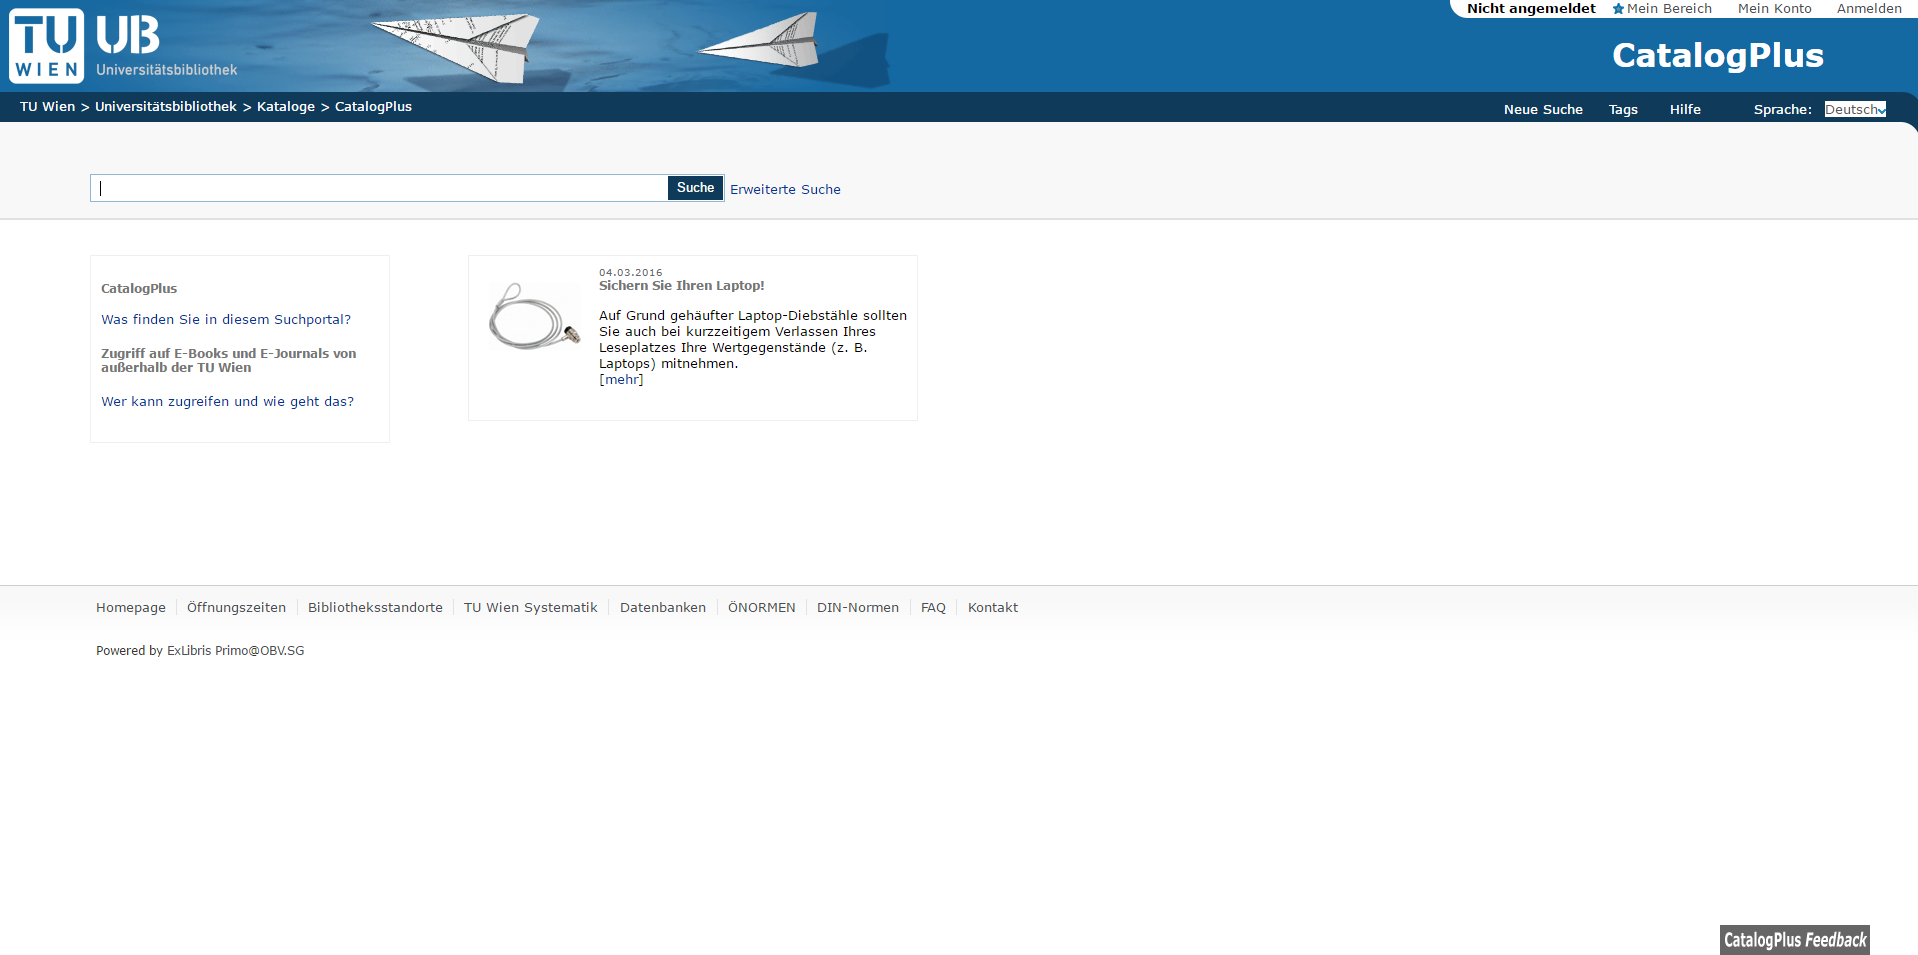
\includegraphics{images/screenshots/screenshot_ub_tu.PNG}}}
\subfigure[Extended search]
{\scalebox{0.3}{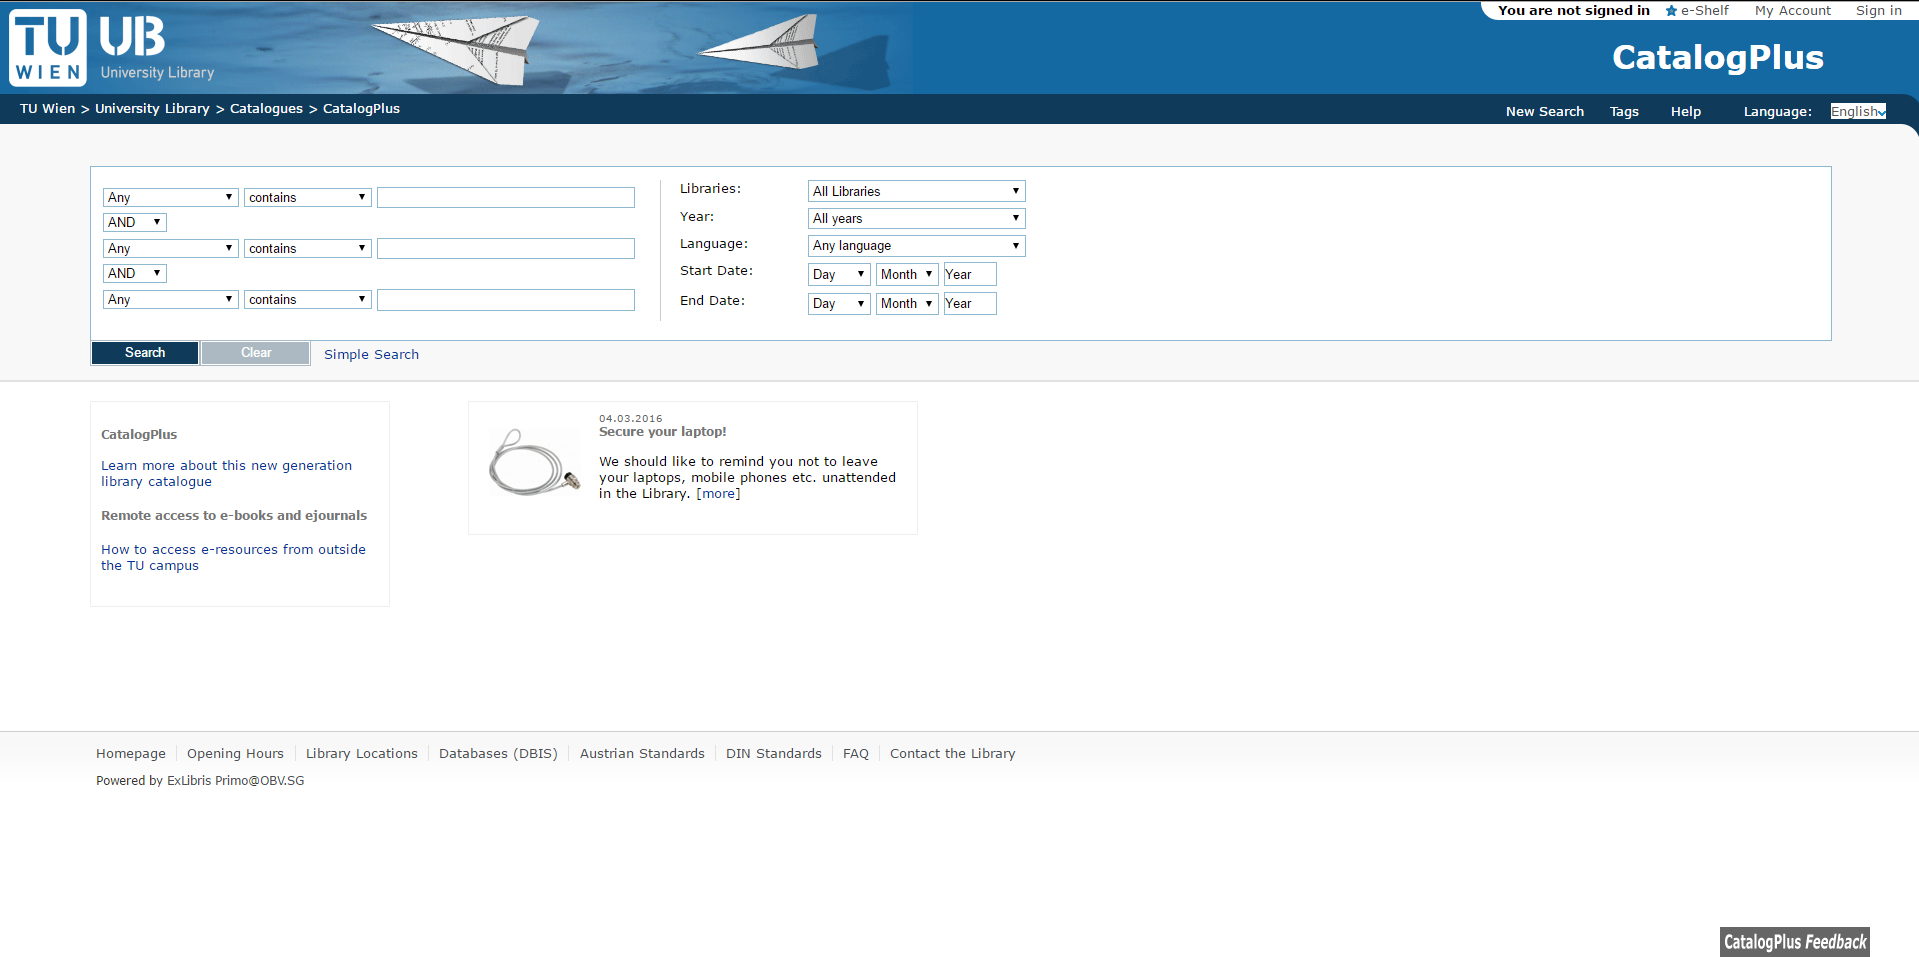
\includegraphics{images/screenshots/screenshot_ub_tu_extended_search.PNG}}}
\caption[Website of the TUVienna library]{Website of the TUVienna library}
\label{Fi:UB_TU}
\end{figure}

\paragraph{Use case}
This question aimed for a use case similar to the project Linked Data Libraries (described in Section ~\ref{ld-libraries}). The proposed scenarios was to publish the data or meta-data of the university library (and all of its specialized libraries) as LOD and provide an application to access the data. A further option of this scenario would be an interlinking to other LOD data sets, e.g. from the publisher ``Springer'' or to other universities like LD4L do it.

\paragraph{Statistically evaluation}
It can be seen in Figure~\ref{Fi:lib-data} that the interviewed persons strongly agreed to the scenario (found it ``extremely useful'') and could imagine a similar project at the TU Vienna. Only one interviewee found it difficult to see advantages and therefore argued that he wouldn't use it. Another one found it indeed useful in a general context but not for his own work.

\begin{figure}[htbp]
\centering
	\begin{tikzpicture}
		\begin{axis}		
			[title=Usefulness of library (meta-)data as LOD,
			ybar,% Balken
			% urspr�ngliche y-Werte unterhalb der Balken:
			nodes near coords,nodes near coords align=above,point meta=rawy,
			axis x line=bottom, axis y line=left,% Achsen nur unten und links,
			%xlabel=blub,ylabel=bla, % Beschriftung der Achsen
			ymin=0,% minimaler y-Wert ist 0
			xtick=data,% xticks nur an Stellen mit Daten
			enlargelimits=auto,% Vergr��ern der R�nder des Diagramms
			% Ausgabe der x Werte ohne Tausendermarkierung@
			x tick label style={/pgf/number format/1000 sep=}]
			\addplot table[x=Question, y=Number] {data/data_ld_library_useful.csv};
		\end{axis}
	\end{tikzpicture}
		\begin{tikzpicture}
		\begin{axis}		
			[title=Imagine at TUVienna? Would use it?,
			ybar,% Balken
			% urspr�ngliche y-Werte unterhalb der Balken:
			nodes near coords,nodes near coords align=above,point meta=rawy,
			axis x line=bottom, axis y line=left,% Achsen nur unten und links,
			%xlabel=blub,ylabel=bla, % Beschriftung der Achsen
			ymin=0,% minimaler y-Wert ist 0
			symbolic x coords = {{No, Yes}},
			xtick=data,% xticks nur an Stellen mit Daten
			enlargelimits=auto,% Vergr��ern der R�nder des Diagramms
			% Ausgabe der x Werte ohne Tausendermarkierung@
			x tick label style={/pgf/number format/1000 sep=},
			legend pos=north west]
			\addplot table[x=Answer, y=Imagine] {data/data_ld_library_use.csv};
			\addplot table[x=Answer, y=Use] {data/data_ld_library_use.csv};
			\legend{Can imagine, Would use}
		\end{axis}
	\end{tikzpicture}
	\caption[Usefulness of library (meta-)data]{Usefulness of library (meta-)data as LOD}\label{Fi:lib-data}
\end{figure}

\paragraph{Needs, potential benefits}
As stated, all of the interviewed persons could imagine a similar project. One of the main reasons of the strong acceptance was the current interface of the library website~\footnote{\url{www.ub.tuwien.ac.at/}}, which only allows a search with only a few, specified parameters (see Figure~\ref{Fi:UB_TU}). Also the physical search in the library itself was claimed due to a lack of orientation and knowledge about the position of e.g. a searched book. Both point of criticism are expected to vanish by an open access to the data and appropriate applications, which provides a detailed and personalizable search interface.\newline
Furthermore an open access to the data was seen as a chance for everyone to interact with it and as opportunity to stimulate creativity of the people.

\paragraph{Barriers, potential disadvantages}

The library institution was very conservative perceived with skepticism, refusals and resentment against new ideas, especially in a technical term. It was stated by some interviewees, that this kind of project would only be seen as an extra amount of work in the library and not as an opportunity.\newline
Beside the expected opposition there was also a real amount of work estimated by the interviewees. In particular there would be an effort to invest in digitizing books and keep this data up-to-date. This would be an important part of the project, otherwise the data would lose there value - not digitized data could not be distinguishable from not available data. Therefore it would be essential to have a complete and current database. \newline
Another concern of the interviewed people were the copyright of the data. However, this problem was seen as handleable, because only meta-data would be open accessible.\newline
At last, one interviewee declined the idea and usefulness of the LD4L and similar projects because of the existing platform Google Scholar~\footnote{\url{www.scholar.google.at/}}. He stated, that it already provides similar data and therefore everything he needs for his work. Further an additional platform would be too intricate to use.

\subsubsection{Data from the Publication database}

\begin{figure}[htbp]
\centering
{\scalebox{0.3}{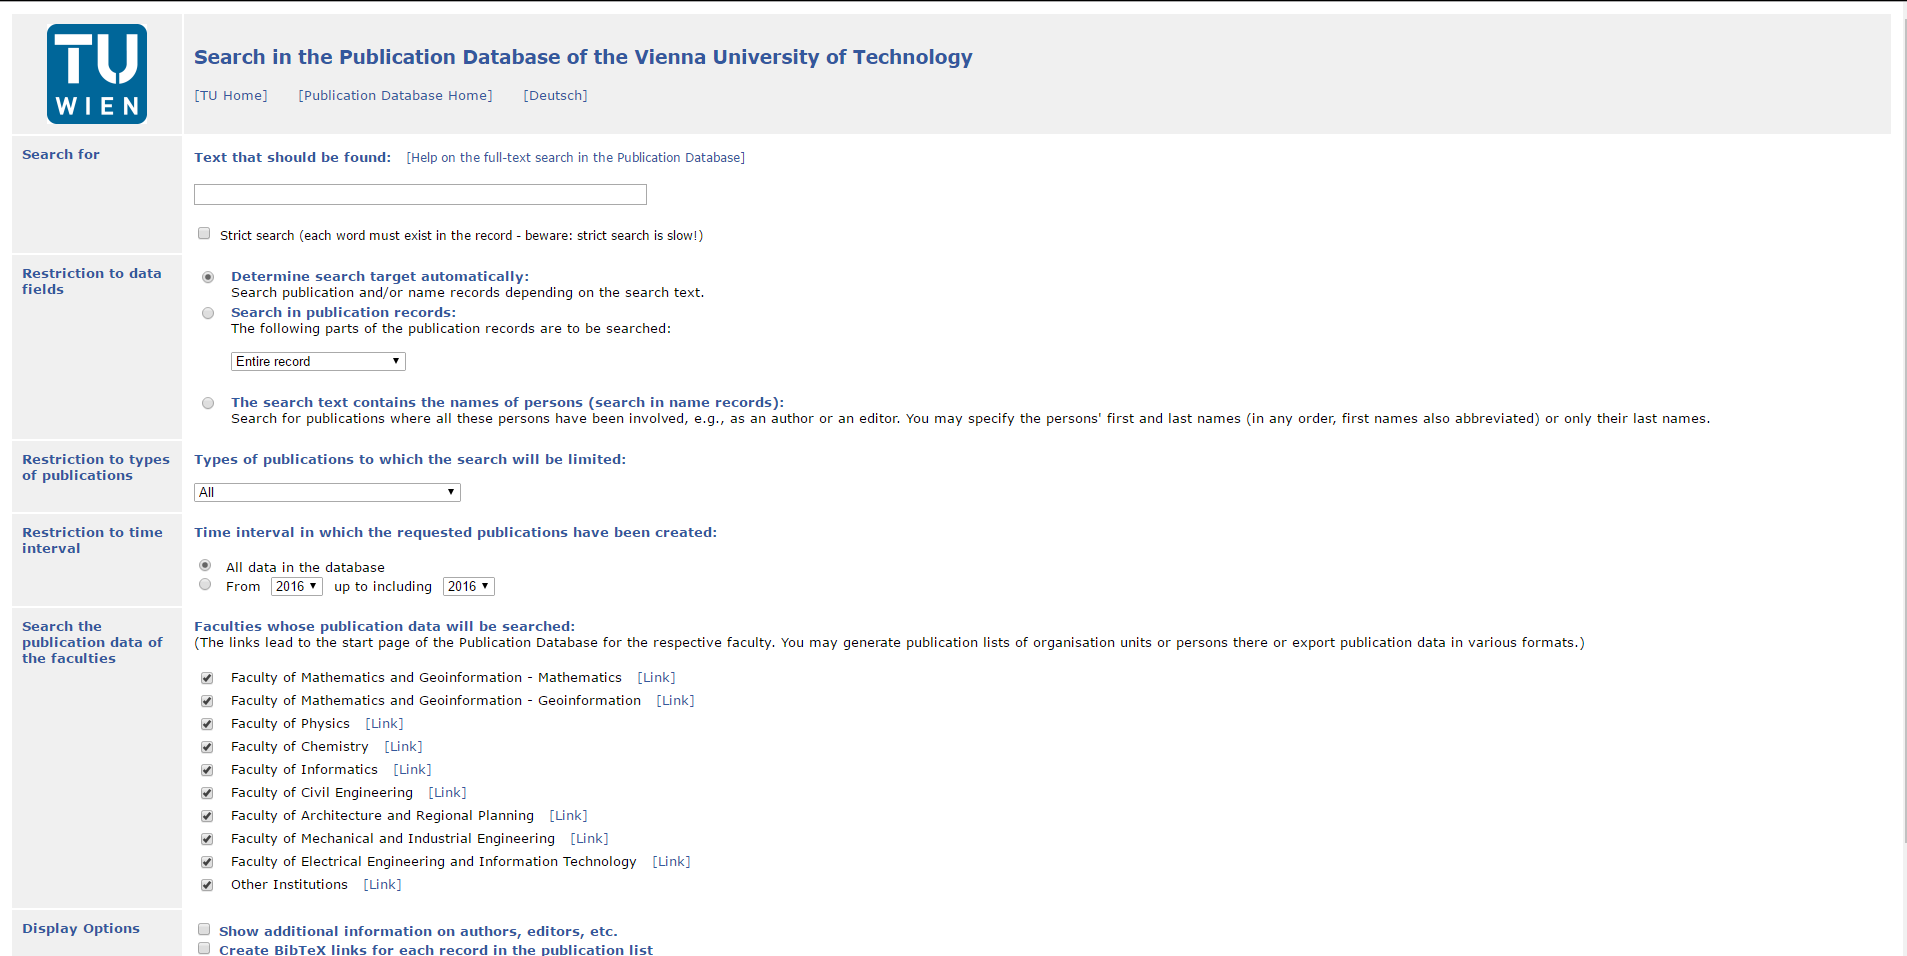
\includegraphics{images/screenshots/screenshot_pub_database.PNG}}}
\caption[Publication database]{Publication database}
\label{Fi:pub_db}
\end{figure}

\paragraph{Use case}\label{section:pub_db_usecase}
The proposed use case applied to the already existing publication database of the university. In the current state the database can be accessed via its website~\footnote{\url{www.publik.tuwien.ac.at/pubstart.php}}, where an interface for search exists. For other search parameters a request to the administration has to be made. The introduced LOD approach provides an LOD interface to the existing database, so the data can be accessed over e.g. SPARQL. This use case follows the principle of the existing ``Open Research Online''~\footnote{\url{http://data.open.ac.uk/page/context/oro}} endpoint from the Open University, which expose information about publications originating from OU researchers using the BIBO Ontology (see section~\ref{subsubsec:ontologies} for details).

\paragraph{Statistically evaluation}
Similar to the library use case the interviewees liked the idea and found it all ``extremely useful''. Everyone could imagine such a project at TUVienna and would also use it.

\begin{figure}[htbp]
\centering
	\begin{tikzpicture}
		\begin{axis}		
			[title=Usefulness of publication data as LOD,
			ybar,% Balken
			% urspr�ngliche y-Werte unterhalb der Balken:
			nodes near coords,
			nodes near coords align=above,
			point meta=rawy,
			axis x line=bottom, axis y line=left,% Achsen nur unten und links,
			%xlabel=blub,ylabel=bla, % Beschriftung der Achsen
			ymin=0,% minimaler y-Wert ist 0
			xtick=data,% xticks nur an Stellen mit Daten
			enlargelimits=auto,% Vergr��ern der R�nder des Diagramms
			% Ausgabe der x Werte ohne Tausendermarkierung@
			x tick label style={/pgf/number format/1000 sep=}]
			\addplot table[x=Question, y=Number] {data/data_publication_useful.csv};
		\end{axis}
	\end{tikzpicture}
		\begin{tikzpicture}
		\begin{axis}		
			[title=Imagine at TUVienna? Would use it?,,
			ybar,% Balken
			% urspr�ngliche y-Werte unterhalb der Balken:
			nodes near coords,
			nodes near coords align=above,
			point meta=rawy,
			axis x line=bottom, axis y line=left,% Achsen nur unten und links,
			%xlabel=blub,ylabel=bla, % Beschriftung der Achsen
			ymin=0,% minimaler y-Wert ist 0
			symbolic x coords = {No, Yes},
			xtick=data,% xticks nur an Stellen mit Daten
			enlargelimits=auto,% Vergr��ern der R�nder des Diagramms
			% Ausgabe der x Werte ohne Tausendermarkierung@
			x tick label style={/pgf/number format/1000 sep=},
			legend pos=north west]
			\addplot table[x=Answer, y=Imagine] {data/data_publication_use.csv};
			\addplot table[x=Answer, y=Use] {data/data_publication_use.csv};
			\legend{Can imagine, Would use}
		\end{axis}
	\end{tikzpicture}
	\caption[Usefulness of publication data]{Usefulness of publication data as LOD}\label{Fi:pub-data}
\end{figure}

\paragraph{Needs, potential benefits}
In contrast to the previous use case, the work amount of work was significant lesser stated, because the data are already there, just as the need of being up-to-date of the database.\newline 
Further some of the interviewed persons (independent to each other) come up with the idea of building an application based on the Linked Open Data interface to provide an overview of a researcher references as a widget or similar for a personal website. The data could be interlinked e.g. with the LOD interface of the Springer publisher~\footnote{\url{www.lod.springer.com/}} and complemented by including the Journal Impact Factor (JIF).

\paragraph{Barriers, potential disadvantages}
The interviewees identified uniformly a problem with the data ownership. Although there is an administration of the database, the \textit{ownership} of the data itself is very unclear and therefore a contact and responsible person would be hard to find for such a project - there needs to be more investigation.\newline
Another point, some of the interviewed persons were concerned of, was quality assurance - to use the data, they need to be synchronized with the original database. To taking care of this point, the implementation of a similar project has to ensure this.

\subsubsection{Other data}
\%\%\%\%tbd\%\%\%\%
\paragraph{Needs, potential benefits, use-cases}
\paragraph{Challenges}

\section{Proposed technical architecture and challenges}
As an organization covering areas like research, student affairs and administration a university has to manage a significant amount of knowledge, adding new information on a daily basis.
Such an application domain is complex and includes areas like management of an academic library and provision of educational resources which have to be conform with stakeholders requirements. Traditionally the \textit{Service Oriented Architectures~(SOA)} have been used to meet these needs. However, as the application domain grows many small and similar services tend to emerge. That phenomena can not only be observed at the Vienna University of Technology, but also at the Open University\footnote{\url{http://www.open.ac.uk/}}~\citet{inproceedings:zablith_consuming_2011}.

A major problem of evolving similar, independent services are diverging data formats and service owners. Thus, knowledge and administrative information that has been collected by multiple services can not be easily interlinked. An example for such isolated services is the e-learning platform called TUWEL\footnote{\url{https://tuwel.tuwien.ac.at/}}, combining moodle\footnote{\url{https://moodle.org/}} and the central information system called TISS\footnote{\url{https://tiss.tuwien.ac.at/}}. These services provide course information and material, but are intended for different purposes. Whereas TISS focuses mainly on administrative functionality, TUWEL supports the interaction between teacher and student. 
Adding additional services which, for example, synchronize deadlines and registration dates is costly due to the fact that the information is separated over different isolated sources and not easily accessible. 

\subsection{The big picture}

\begin{figure}[htbp]
\centering
{\scalebox{0.7}{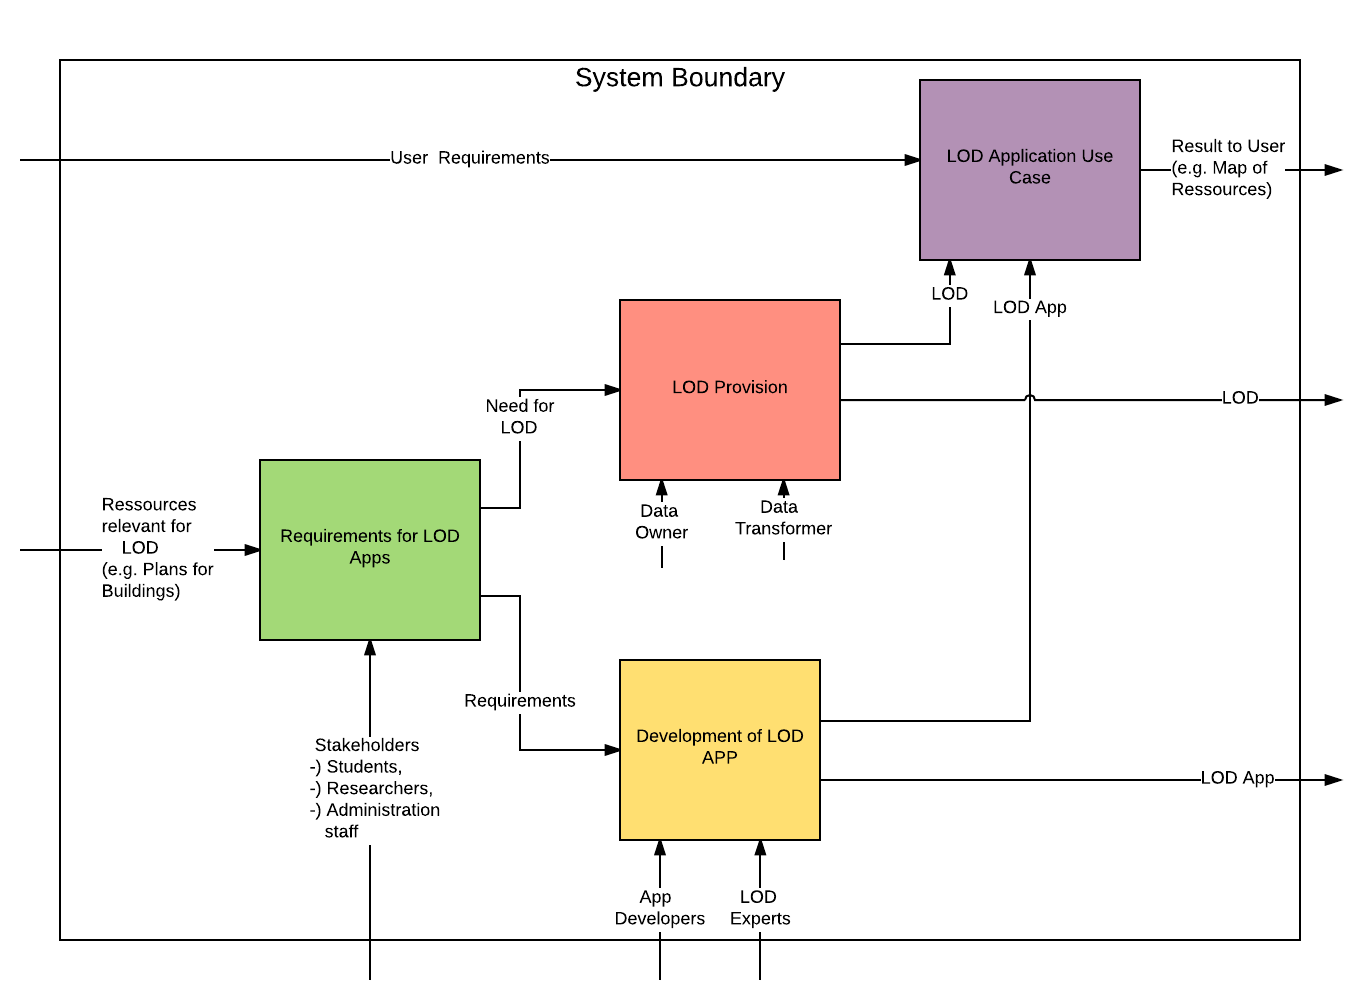
\includegraphics{images/architecture/idef0.png}}}
\caption[High level framework for LOD publishing]{High level framework for LOD publishing in IDEF0 notation}
\label{Fi:idef0}
\end{figure}
\subsubsection{Parts}
In this sub-section we provide an overview of a high level architecture, illustrated
in Figure~\ref{Fi:idef0}, for a university wide publication framework which includes:

\begin{itemize}
	\item \textbf{Requirements for LOD-Applications}\newline
	At the beginning stand the existing resources and the needs of the stakeholder. Combining these leads to the requirements for an application, the first step of the process. According to this requirement a decision has to be made whether they are  realizable depending on the cost-value ratio and whether the solution has to be a LOD application. These process has to actively involve all stakeholders.
	\item \textbf{Data Provision}\newline
	After defining the requirements, the existing data (e.g. a publication database) must be transformed in a appropriate, machine readable LOD format. These can happen in a manually (only for small data sets) or a (semi-)automated (for big data set) way. Ideally there is a automated transformer based on an existing, well maintained and up-to-date database so there has to be less cared about the of the data (for a more technical description see Section~\ref{subsubsec:sources}). Key roles for this process are the original data owner and the data transformer.
	\item \textbf{Development of an Application}\newline
	Based on the requirements definitions from the previous step a proper application (e.g. a browser of publication data) now can be constructed considering the stakeholder needs and existing resources (transformed to LOD).  To support this process and to not obtaining all knowledge from zero it is recommended to access the knowledge of LOD experts (e.g. provided by the LinkedUniversities~\footnote{\url{www.linkeduniversities.org/}}). The development can simultaneously be done with the data provision if proper interface between the application and its data are made. 
	\item \textbf{Application Use Case}\newline
	Combining the data, transformed in LOD, the LOD application and user requirements (not the application requirements from the first step) result in the actual application use case, representing the environment or the domain.
\end{itemize}

\subsubsection{In- and outbound interfaces}

There were several indirectly interfaces mentioned above - we define them now in a more formal way and divide them in inbound (arrows pointing from outside the system boundary) and outbound interfaces (arrows pointing from inside the system boundary).

The inbound interfaces are:

\begin{itemize}
	\item \textbf{User Requirements}\newline
	Understanding user requirements is an essential part of the software development process. Due to the open nature of Linked Open Data privacy concerns and legal issues should be already considered in the requirements as misunderstandings are hard to fix in later phases.
	\item \textbf{Existing Resources}\newline
	The starting point of every LOD application are resources, ideally already existing (to reduce the amount of work). It can be everything from relational databases, simple Excel files or other Linked (Open) Data sets. For more details see section~\ref{subsubsec:sources}.
	\item \textbf{Stakeholders}\newline
	Stakeholders are defined as \textit{"`a person, group or organization that has interest or concern in an organization. Stakeholders can affect or be affected by the organization's actions, objectives and policies."'}~\citet{book:Post2002} Their needs and demands have to be considered in a LOD project as similar as in every other software project.
	\item \textbf{Application Developers}\newline
	\item \textbf{LOD Experts}\newline
	To avoid unnecessary redundancy in acquiring knowledge of LOD implementation, it is highly recommended to involve either LOD experts in the development or access their accumulated know-how e.g. by platforms like LinkedUniversities~\footnote{\url{www.linkeduniversities.org/}} (see section~\ref{linkeduniversities})
	\item \textbf{Data Owner}\newline
	Every data set has its owner, therefore this role has to be considered in the development process to avoid organizational conflicts and copyright issues. Ideally he is directly involved to access his specific know-how about the data set.
	\item \textbf{Data Transformer}\newline
	To use a data set in a LOD approach, the data have to be transformed either manually or (semi-)automatically into a proper format (see~\citet{artivle:bernerslee-t-2006-1} for the 5 star model of data format and section~\ref{subsubsec:sources} for details about transformations).
\end{itemize}

The outbound interfaces are:

\begin{itemize}
	\item \textbf{Linked Open Data}\newline
	As a result of the LOD provision the actual data are provided e.g. as SPARQL endpoint, so others can easily access and use them in other applications. For technical details about endpoints see section~\ref{subsubsec:provision} or as example the SPARQL endpoint of The Open University~\url{www.data.open.ac.uk/query}.
	\item \textbf{Application}\newline
	The outcome of the development phase are applications for end-users to access and interact with the data e.g. in form of an web platform. For technical details about endpoints see section~\ref{subsubsec:provision} or as example the application list of The Open University~\url{www.data.open.ac.uk/applications.html}.
	\item \textbf{End-User Result}\newline
	Finally the main result is the actual interaction of the users with the applications and endpoints, (hoepfully) acting in the boundaries of the defined use cases.
\end{itemize}

\newpage

\subsection{Proposal of a technical architecture}
In this section we will briefly describe a proposal technical architecture for publishing (existing) data as Linked Open Data
% with the help of the example use case "`publication data as LOD"' (see section~\ref{section:pub_db_usecase})
. The proposal is mainly inspired by the toolkit "`Tabloid"' ("`Toolkit ABout Linked Open Institutional Data"') by the LUCERO Project~{\footnote{\citet{url:lucero-tabloid}} - a collection of tools, examples and documentions. The general principle is a system, which extract RDF data from existing data sources (section~\ref{subsubsec:sources}), load them into a triple store (section~\ref{subsubsec:store}) and finally expose them to the web (section~\ref{subsubsec:provision}). For illustration see the LUCERO workflow in figure~\ref{Fi:lucero_architecture} (in this part only the generic parts are described). In this workflow there are way more components than we will talk about (e.g. mechanism of detecting data changing) than shown in the figure. Additional a more generic architecture can be seen in figure~\ref{Fi:tec_architecture}.
%url:linked-universities-vocabularies
%url:linked-universities-tools
%url:lucero-tabloid

\begin{figure}[htbp]
\centering
{\scalebox{0.5}{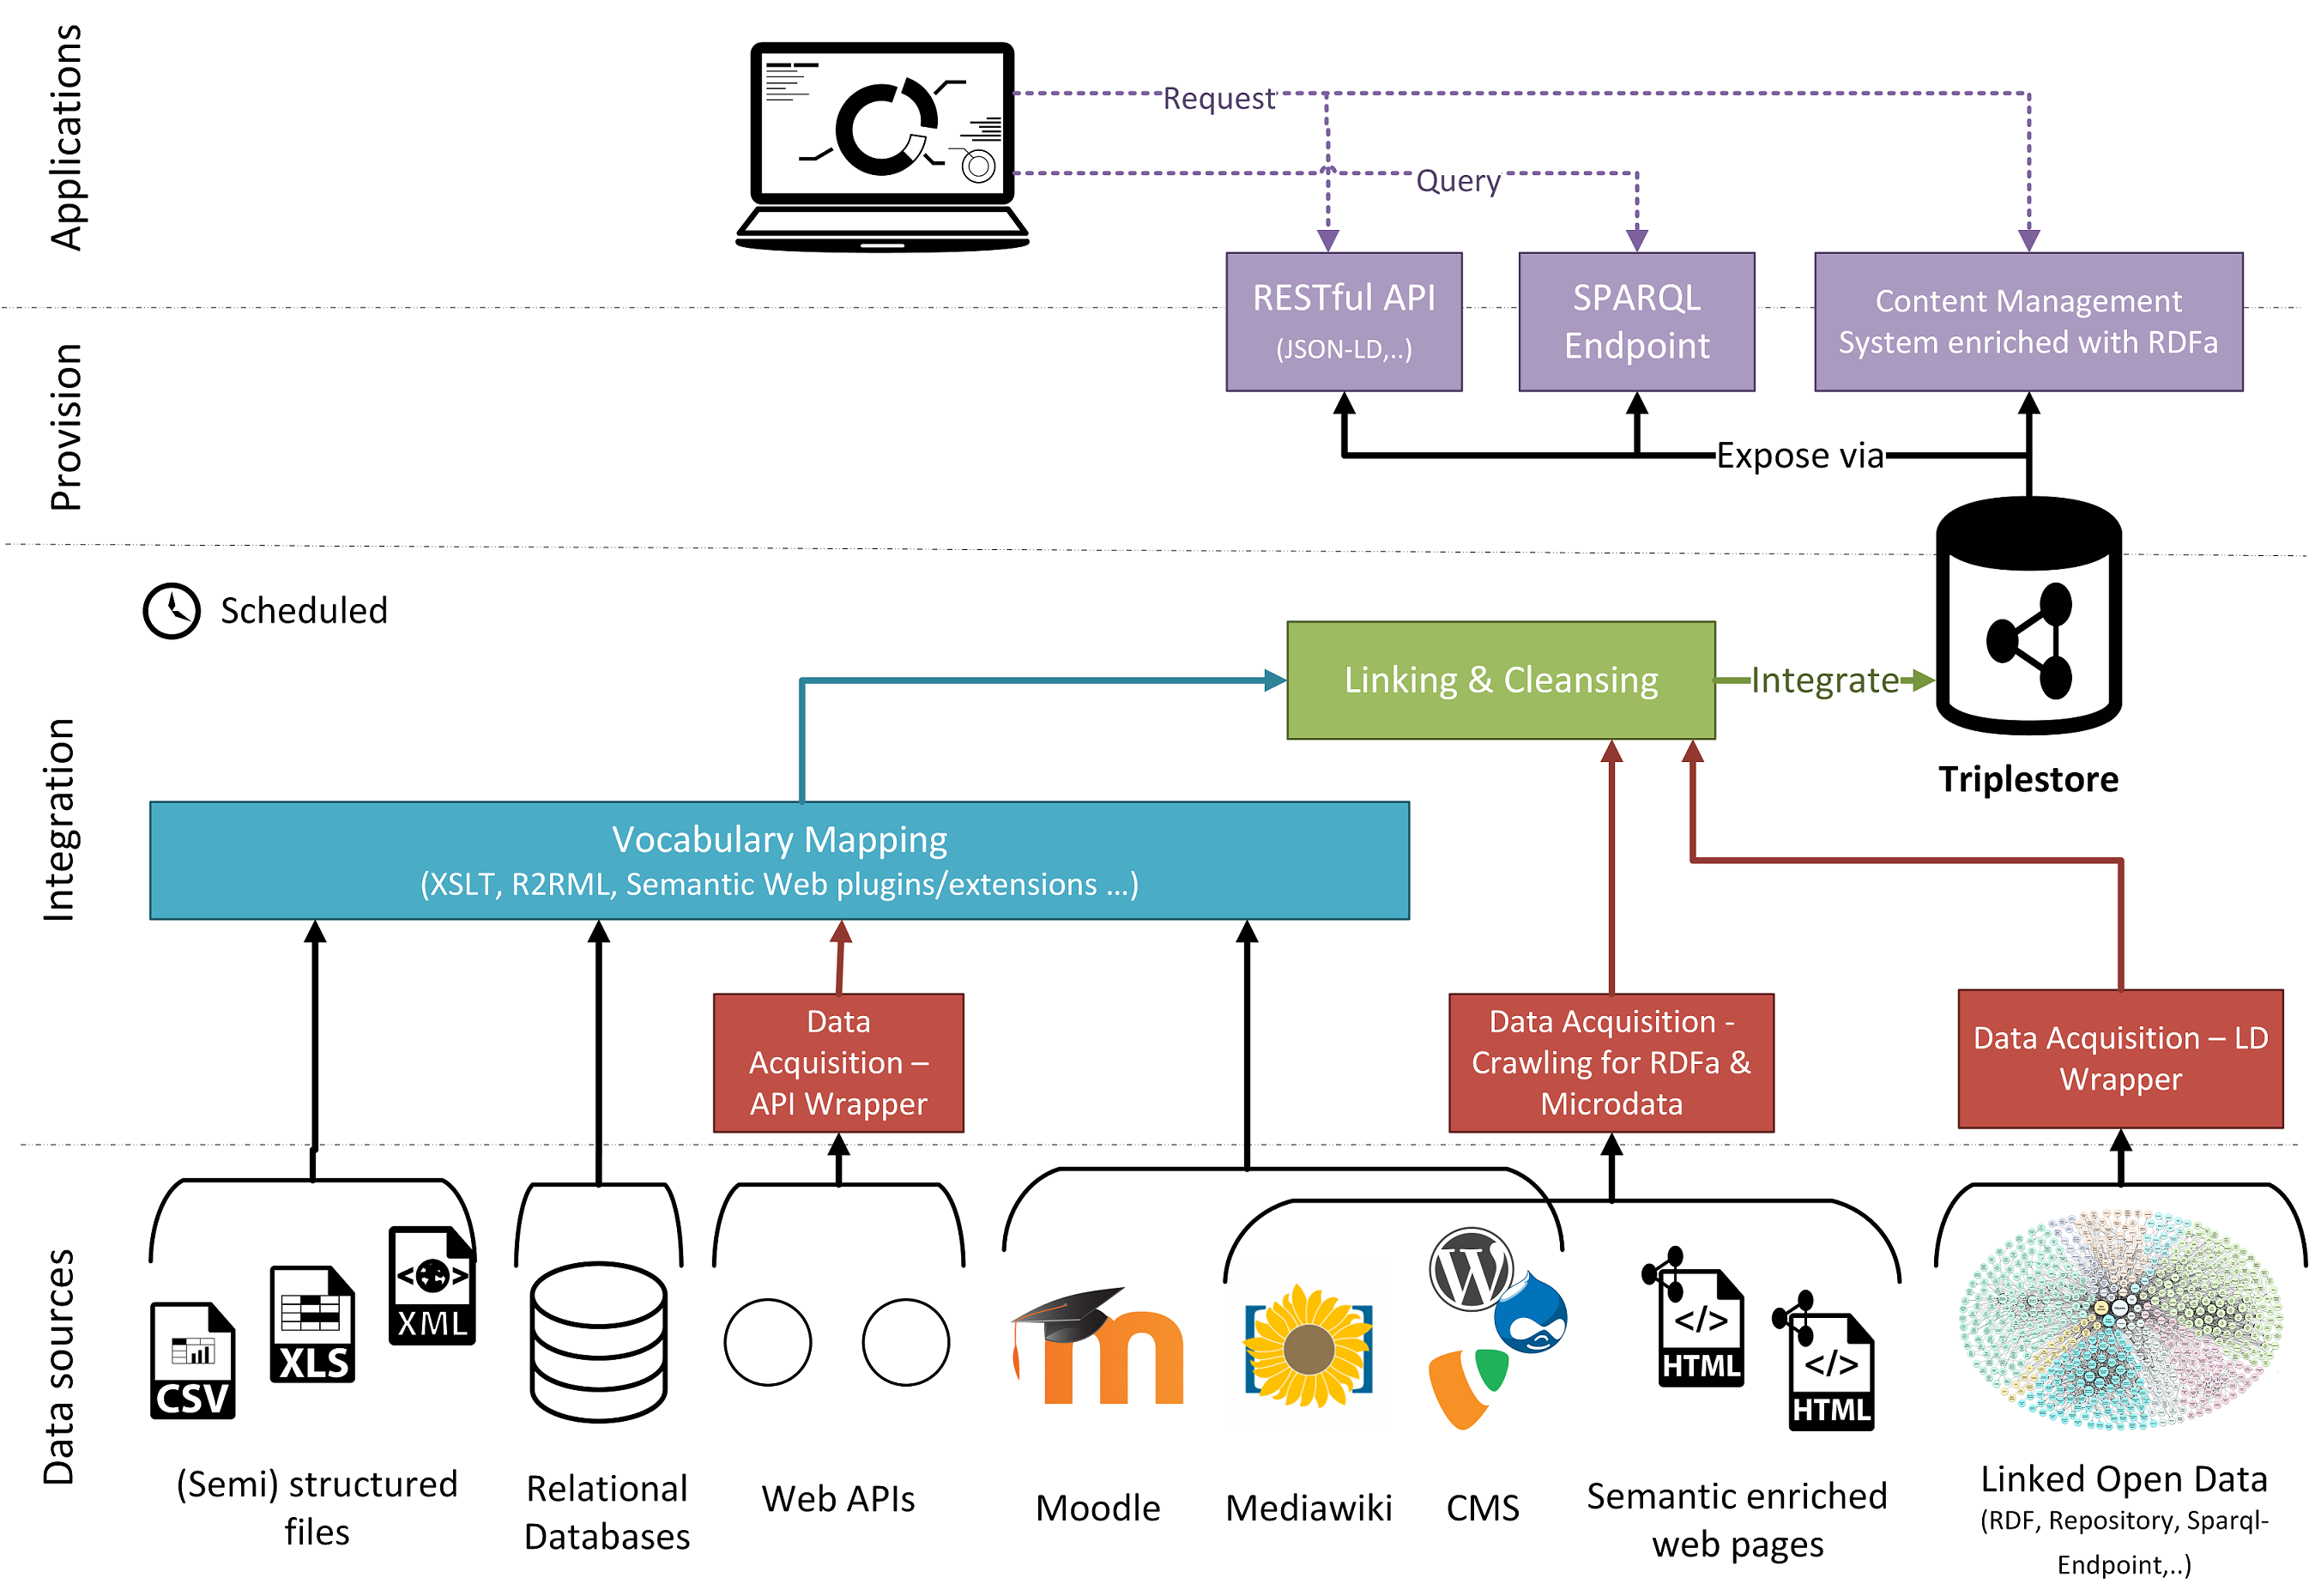
\includegraphics{images/architecture/lod_technical_architecture.png}}}
\caption[Generic high level technical architecture of a LOD system]{Generic high level technical architecture of a LOD system //TODO: source}
\label{Fi:tec_architecture}
\end{figure}
\begin{figure}[htbp]
\centering
{\scalebox{0.13}{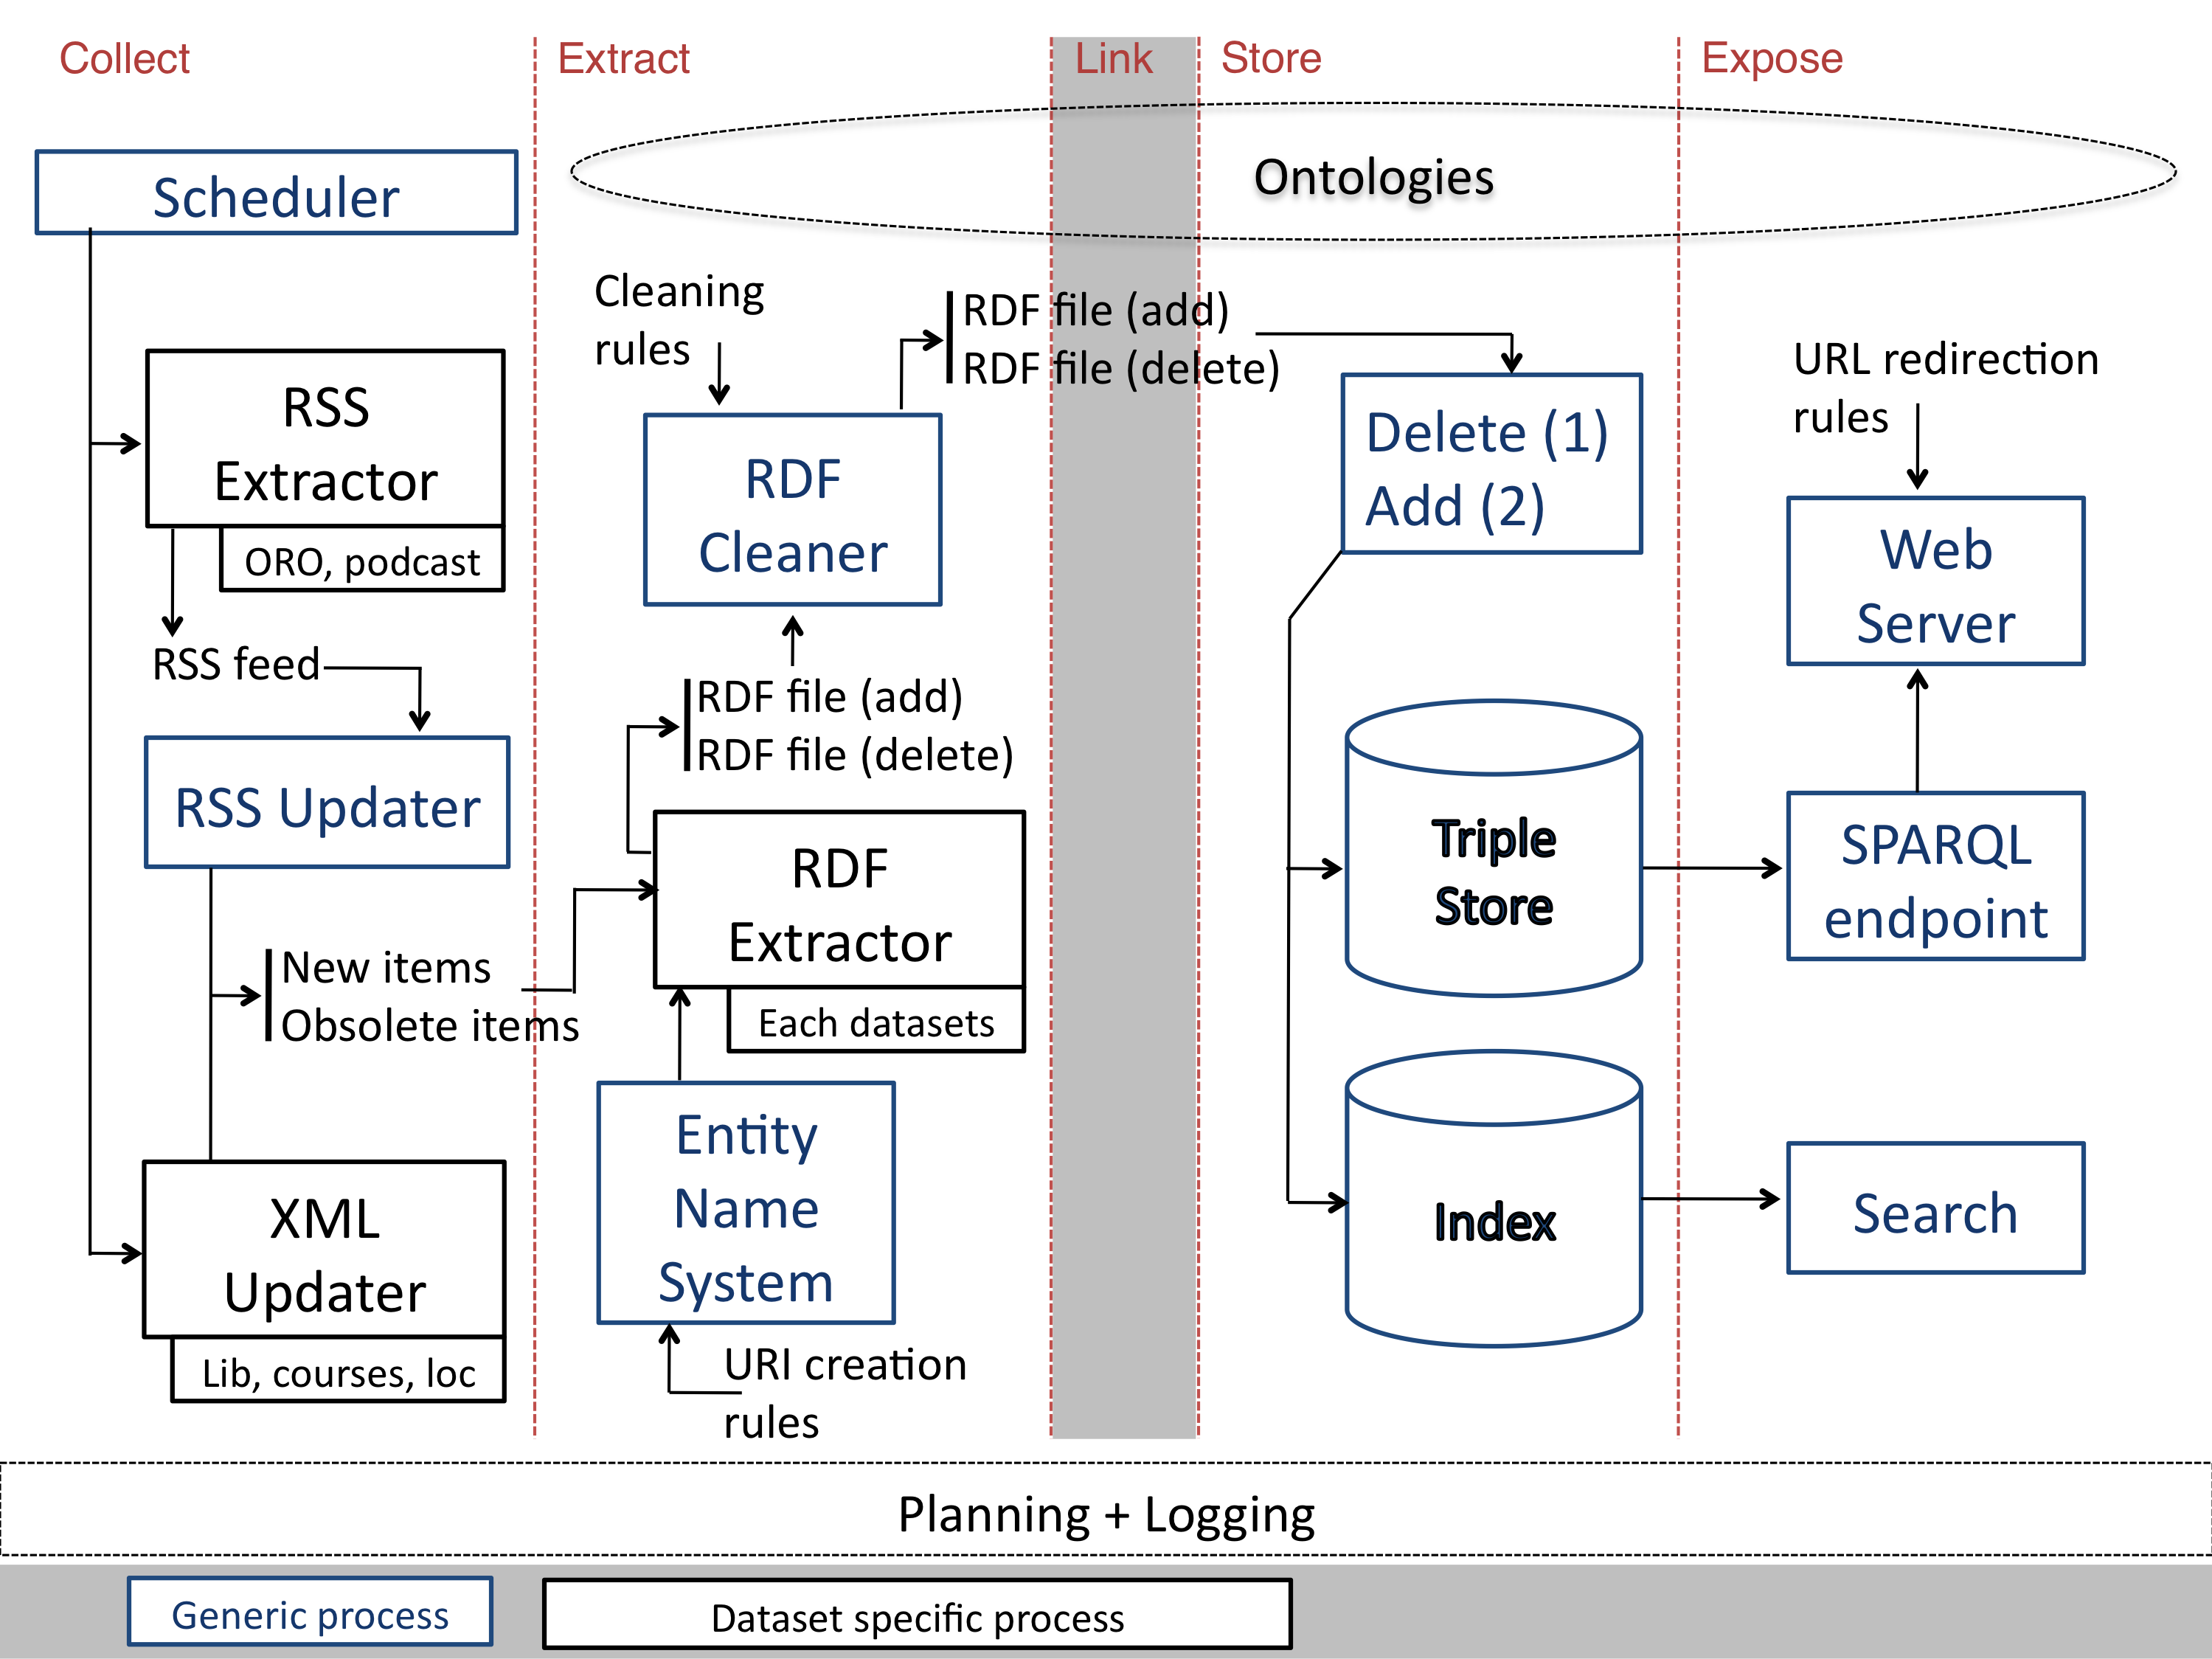
\includegraphics{images/architecture/lucero-workflow.png}}}
\caption[Example: the LUCERO workflow]{Example: the LUCERO workflow\footnote{\citet{url:lucero-tabloid}}}
\label{Fi:lucero_architecture}
\end{figure}

\subsubsection{Collect \& extract data from sources}\label{subsubsec:sources}
The first step must be to collect and extract the data from the source and transform them into a proper LOD format, e.g. RDF. By now there are basically for every data format tools for transforming them into RDF, LinkedUniversities made a collection of them~\footnote{\url{http://linkeduniversities.org/lu/index.php/tools/index.html}}, here are the main tools:

\begin{itemize}
	\item \textbf{From Relational Databases}
	\begin{itemize}
		\item \textbf{Triplify}~\footnote{\url{http://triplify.org/}} is a tool which use SQL queries to generate RDF data from a relational database.
		\item \textbf{D2RQ}~\footnote{\url{http://www4.wiwiss.fu-berlin.de/bizer/d2r-server/}} is a tool which also use SQL queries but with the use of a mapping that relates the structure of a database to RDF triples. It transformers SPARQL queries at run-time into SQL queries using this mapping.
	\end{itemize}
	\item \textbf{From XML and RSS}\newline
	In terms of syntax, XML, RSS and RDF sharing the same base, so there have to be fewer effort to be done to transform them syntactic, commonly using XSLT. W3C recommended the GRDDL~\footnote{\url{http://www.w3.org/TR/grddl/}} language for this purpose.
	\item \textbf{From Tables and Spreadsheets}
	\begin{itemize}
		\item Google Refine~\footnote{\url{http://code.google.com/p/google-refine/}} with the RDF Extension~\footnote{\url{http://lab.linkeddata.deri.ie/2010/grefine-rdf-extension/}} is an easy way to clean, transform and explore data in a tabular format including MS Excel, Google Spreadsheet and CSV.
		\item Other tools like Any23~\footnote{\url{http://lab.linkeddata.deri.ie/2010/grefine-rdf-extension/} (at the moment of the work unavailable)} or QUIDICRC~\footnote{\url{http://any23.org/}(at the moment of the work unavailable)} providing simple transformation from CSV to RDF
	\end{itemize}
\end{itemize}

After extracting the data as RDF from there source, they need to be cleaned and interlinked with themselves and other data.

\subsubsection{Vocabularies and Ontologies}\label{subsubsec:ontologies}
To represent and store the collected data, they must be mapped into an ontology and a vocabulary.

\citet{jour:gruber} defines an \textit{ontology} as "'\textit{an explicit specification of a conceptualization}"'.
\textit{Conceptualizations} are objects, entities or concepts that may or may not exist in the universe. In addition to that, the \textit{vocabulary} defines the relationships between those objects. In other words, the vocabulary defines the conceptual model of what can be represented. 
\citet{jour:owl} describe ontologies from a more practical point of view defining the three conceptual components of an ontology - \textit{classes}, \textit{instances} and \textit{properties}. Regardless of what concrete implementation of an ontology is used graphical representations~(e.g. graph) are preferred over textual ones to give a high level overview of the concepts used in an ontology. 

Again, LinkedUniversities listed a lot of useful vocabularies and ontologies on their website~\footnote{~\url{http://linkeduniversities.org/lu/index.php/vocabularies/index.html}}. As an example for such an ontology let's take a look at the use case "`publication database"' from section~\ref{section:pub_db_usecase}. To mapping the data from this database a bibliographic ontology is needed. LinkedUniversities recommend the BIBO (Bibliographic Ontology)~\footnote{~\url{http://bibliontology.com/}}. It can be used as a citation ontology, as a document classification ontology, or simply as a way to describe any kind of document in RDF, so it is ideally for this purpose. You can see the BIBO graph in figure~\ref{Fi:bibo_graph}.

\begin{figure}[htbp]
\centering
{\scalebox{0.5}{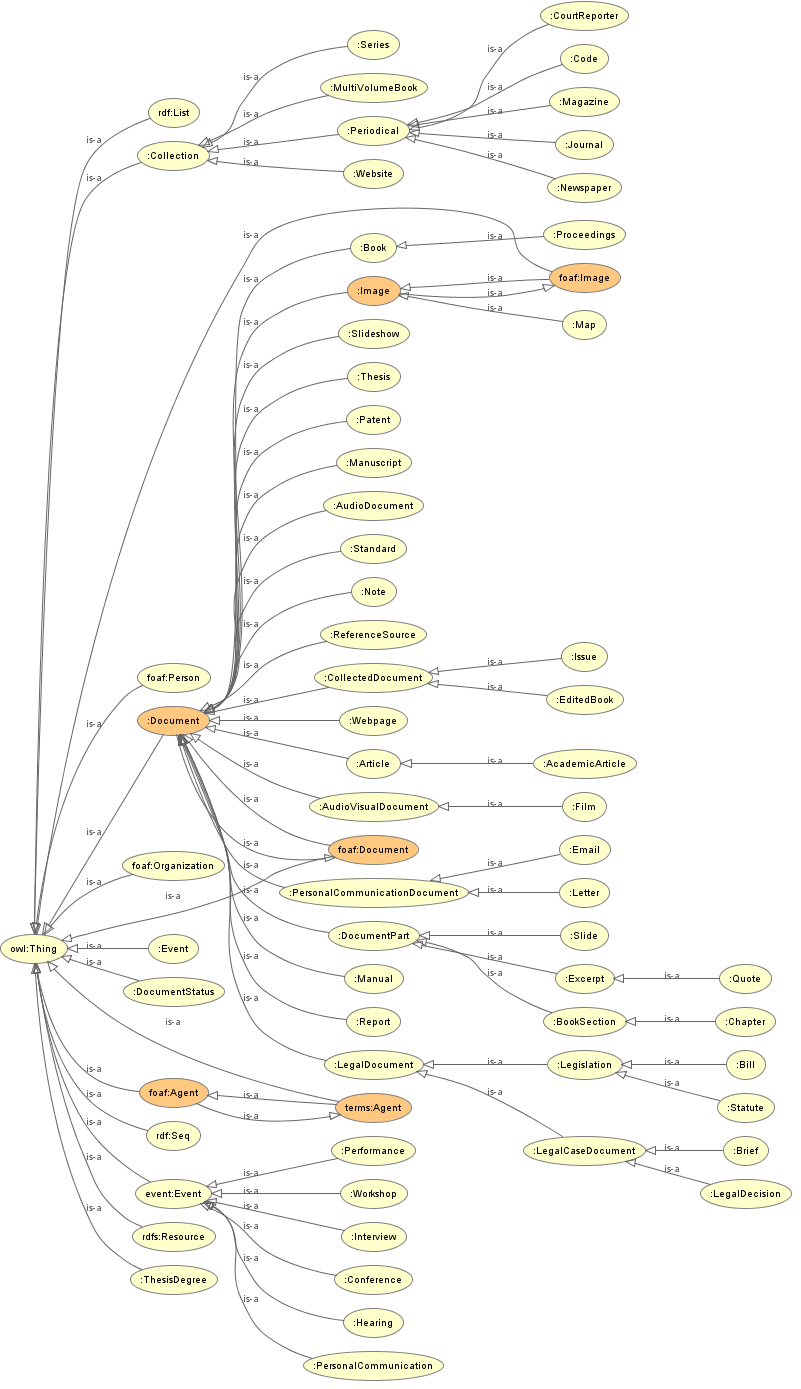
\includegraphics{images/architecture/bibo_graph_2.png}}}
\caption[The BIBO graph]{The BIBO graph}
\label{Fi:bibo_graph}
\end{figure}

%\subsubsection{Link the data}\label{subsubsec:link_data}
%Another crucial element concerns the way the different datasets connect to each other. 
\subsubsection{Store the data}\label{subsubsec:store}
Considering the performance of such a system and to avoid too much communication with the original data source, the center of the system is a triple store, where the extracted data are stored and from there exposed to the web. A triple store (or RDF store) is a purpose-built database, \textit{"`designed to store and retrieve identities that are constructed from triplex collections of strings (sequences of letters). These triplex collections represent a subject-predicate-object relationship that more or less corresponds to the definition put forth by the RDF standard."'}~\citet{url:triplestore}. There are a lot of implemenations of such a triple store, like 
Sesame~\footnote{\url{http://rdf4j.org/}}, 
Jena TDB~\footnote{\url{http://openjena.org/TDB/}}, 
4Store~\footnote{\url{http://4store.org/}} or 
SwiftOWLIM~\footnote{\url{http://www.ontotext.com/owlim/}}. The LUCERO project settled for the SwiftOWLIM, because it is "`\textit{free, scalable and efficient, and includes limited reasoning capabilities, which might end up being useful in the future}"'~\citet{url:lucero-tabloid}.

\subsubsection{Expose the data to the Web}\label{subsubsec:provision}
The last step is obviously to expose the data from the triple store to the web. For this purpose a SPARQL endpoint is commonly used, but there are also other way, e.g. resolvable URIs, the linked data API~\footnote{\url{http://code.google.com/p/linked-data-api/}} or an Open RESTful API. All of them make the data available so others can query and access them to use it for their application or to serve themselves as resource for linking it with other data.

%\subsection{Stakeholder specific issues (datasets, application types)}
\subsection{Challenges}
\subsubsection{Data ownership}
\subsubsection{Data quality}
\section{Conclusions and future work}~\label{section:conclusion}

Revisit each research question and give a condensed answer derived from possibly multiple methods (e.g., benefits: as identified in interviews, as seen at other universities)

The high-level goal of this work in to enhance and improve processes at the Vienna University of Technology. We have broken down this goal into four distinct research questions:

\begin{itemize}
	\item \textit{RQ1: What are best practices regarding the applicability of Linked Open Data in university settings?}
	\item \textit{RQ2: What are major benefits and barriers for each stakeholder and what are useful use cases?}
	\item \textit{RQ3: What are major challenges for the implementation of a Linked Open Data solution?}
	\item \textit{RQ4: How would a prototypical implementation of a publication framework based on Linked Open Data look like?}
\end{itemize}

In the first part of this paper (section~\ref{section:related_work}) we investigated the first research question and provided international best practices and success stories in educational environments. We have seen that there are plenty similar project and collected knowledge on which a project at the Vienna University of Technology could build on. The Linked Universities provide a wide range of best practices of technologies and ontologies and we presented other successful projects that show the possibilities and benefits of LODs.

In the second part (section~\ref{section:benefits}) we focused on benefits and challenges regarding the applicability as well as the implementation of Linked Data principles for researchers at the Vienna University of Technology by conducting interviews, addressing the second and the third research question. We have seen that a LOD project would be highly welcomed by researcher and that there are a lot of possible use cases. Also the opportunity to develop new ideas based on an access to open data was very common welcome.

In final part (section~\ref{section:technical_architecture}) we addressed research question four by giving a high level overview of a publication framework for educational resources at first (subsection~\ref{section:publication_framework}) and then providing a general architecture for applications built following Linked Data principles (subsection~\ref{subsection:proposal_technical_architecture}). We showed how the best practices presented by the Linked Universities and the Tabloid from the LUCERO project could used to build a system providing LOD. Further we identified major challenges (subsection~\ref{subsec:tec_challenges}) like data ownership, data administration and maintenance that has to be faced when implementing a system similar to the proposed one.

\subsection{Future work}~\label{subsection:future_work}

\subsubsection{Feasible use cases}

As evaluated through the interviews the publication database would be an ideal starting point of a LOD system at the university to demonstrate the benefits of Linked Open Data while the costs and effort of the implementation stay low because the data already exists and are maintained. It would not require additional work by the data provider (e.g. researcher) to deliver the data to the database. Instead the challenge of the data ownership has to be addressed and solved.

On the other hand implementing the library data into a LOD system may face resistance inside the library and has to be done as corporation work with the OBVSG. Therefore a project with all or the majority of the OBVSG may make more sense and probably magnify the benefits (while facing the same challenges).

Similar is valid for the project ideas mentioned in subsection~\ref{subsubsec:further_use_cases}, most of them may make more sense in a Austria- and/or European-wide context.

\subsubsection{General findings about LOD and implementations}

As identified in the interviews, the challenge of data quality and maintenance are very important for any kind of work with LOD. Therefore we recommend using already existing (and therefore maintained) data when starting a LOD project at the university. Gain extra data only for providing LOD may result in more amount of work in building new organization forms to administrate them. When progressing and extending the project it will be easier to reference onto an existing and well working system to convince skeptical people to build the required providing systems and organization forms.

Further, as described in subsection~\ref{subsubsection:general_results}, we advocate to involve students as parts of university courses and project as soon as there are Linked Open Data available to develop new ideas, use cases and applications on base of this data. This would not only produce new application for demonstration but also attract attention on the interfaces.

\section{Acknowledgments}
The authors would like to thank Assoc. Prof. Dr. Stefan Biffl and Dr. Marta Sabou for initializing and support this work, providing necessary feedback and 	tutoring in the context of the seminar ``Wissenschaftliches Arbeiten'' (``Scientific Work'').

Further thanks goes to the participant of the case study, for their time and thoughts.

\section{Acknowledgments}
The authors would like to thank Assoc. Prof. Dr. Stefan Biffl and Dr. Marta Sabou for initializing and support this work, providing necessary feedback and 	tutoring in the context of the seminar ``Wissenschaftliches Arbeiten'' (``Scientific Work'').

Further thanks goes to the participant of the case study, for their time and thoughts.

\cleardoublepage
\phantomsection
\addcontentsline{toc}{section}{References}
\bibliographystyle{plainnat}
\bibliography{references}
\newpage

\begin{appendices}
	\subsection{Questionaire}
	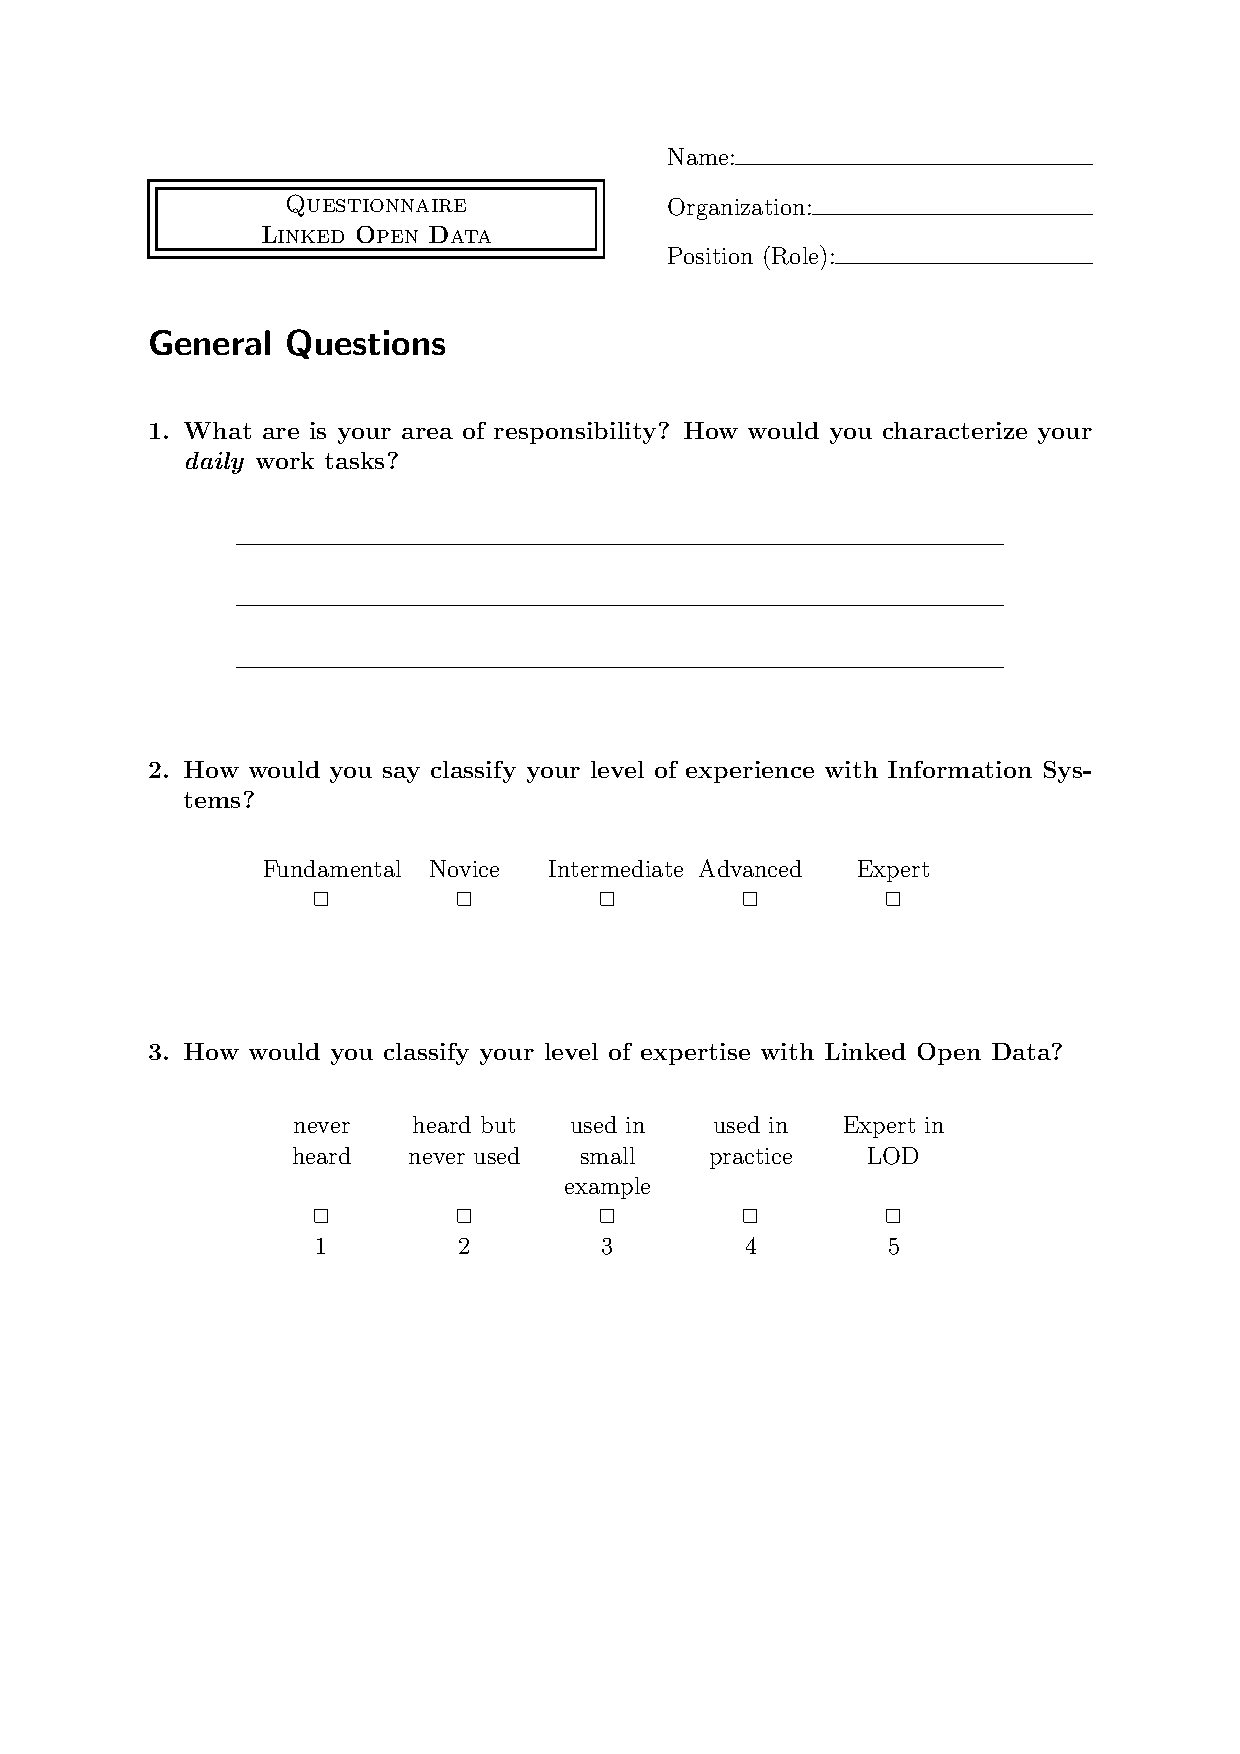
\includepdf[pages=-]{questionaire/questionnaire.pdf}
	\newpage
	\subsection{Contact persons for further investigations}
	\newpage
\end{appendices}
\end{document}
